\chapter{Numerical methods}

\graphicspath{{images/numerical_methods/}}

\section{Lare1D}

LARE, an abbreviation of LAgragian-REmap, is a numerical scheme used to solve partial differential equations like those found in fluid dynamics and magnetohydrodynamics. The core idea of the scheme is to solve the equations on a grid in Lagrangian form, which involves a deformation of the grid, and then to remap the variables back to the original, Eulerian grid. This two-step process, combined with additional shock-capturing techniques such as flux limiters and shock viscosity, is extremely effective at capturing the kind of shocks that are generated in highly compressible, dynamic coronal simulations. It compares extremely well to Roe solvers when solving identical problems~\cite{arberStaggeredGridLagrangian2001}.

As a consequence of the Lagrangian step, the equations are solved in a much simpler form than if they were to be solved in equivalent Eulerian form. The disadvantage of this is that a complex remap step must be introduced. However, once the remap problem is solved, and it is only a complicated but tractable problem of geometry, it is not necessary to change the step when the physics are changed. Like other finite-volume methods, the method requires only local communication, that is a computation on a single cell requires only information from nearby cells. This locality reduces the overhead associated with communication between nodes when implementing the method on large clusters and makes the method viable for large-scale simulations. 

Here, we present the implementation and tests of a 1D LARE scheme applied to the inviscid, compressible Euler equations. We then provide an summary of the MHD code Lare3D~\cite{arberStaggeredGridLagrangian2001} which is used to perform the numerical experiments detailed in the rest of the thesis. 

\subsection{The physical model}
For an ideal, inviscid fluid we use the 1D Euler equations, describing the change in density $\rho$ due to expansion or compression of the fluid through spatial change in the flow velocity $u$,
\begin{equation}
  \frac{D \rho}{Dt} + \rho\frac{\partial u}{\partial x} = 0,\\
  \label{eqn-lare1d-density}
\end{equation}
the change in velocity due to a difference in pressure $p$,
\begin{equation}
  \frac{D u}{Dt} + \frac{1}{\rho}\frac{\partial p}{\partial x} = 0,\\
  \label{eqn-lare1d-velocity}
\end{equation}
the change in internal energy $\varepsilon$ due to expansion or compression,
\begin{equation}
  \frac{D \varepsilon}{Dt} + \frac{p}{\rho}\frac{\partial u}{\partial x} = 0,\\
  \label{eqn-lare1d-energy}
\end{equation}
and an ideal equation of state,
\begin{equation}
  p = \varepsilon\rho(\gamma - 1).
  \label{eqn-lare1d-equation-of-state}
\end{equation}
Including an equation of state simplifies the problem and negates the need to solve the density equation directly. Use has been made of the Lagrangian derivative, defined as
\begin{equation}
  \frac{D }{Dt} \equiv \frac{\partial}{\partial t} + (\vec{u} \cdot \nabla).
\end{equation}
It describes how a quantity within a parcel of fluid changes as that parcel is advected by the flow. 

\subsection{Discretisation} 

\begin{figure}[t]
    \hfill
    \begin{subfigure}{0.3\textwidth}
      \centering
      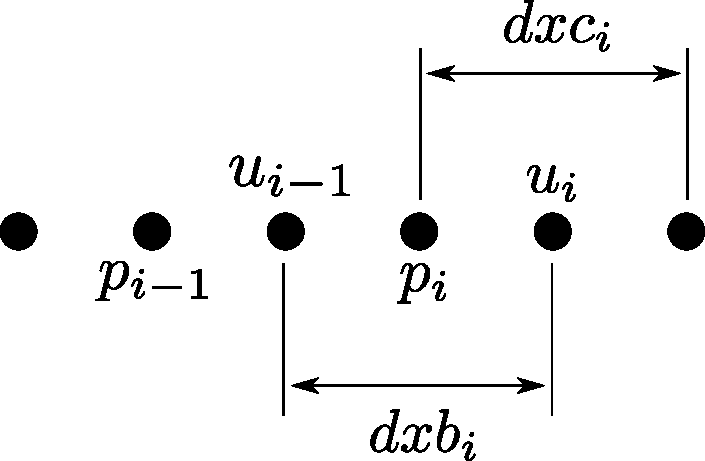
\includegraphics[width=1.0\linewidth]{staggered_grid.pdf}
      \caption{Staggered grid}%
      \label{fig:staggered_grid}
    \end{subfigure}
    \hfill
    \begin{subfigure}{0.49\textwidth}
      \includegraphics[width=\linewidth]{remap.png}
      \caption{Remap step}%
      \label{fig:remap}
    \end{subfigure}
    \caption{\ref{fig:staggered_grid} Staggered grid showing velocity located at cell-boundaries and pressure located at cell-centres, and~\ref{fig:remap} illustration of the deformation of the grid during the Lagrangian step and the remapping of variables back to the original grid during the remap step.}
\label{fig:grid_and_remap}%
\end{figure}

As illustrated in figure~\ref{fig:staggered_grid}, the grid on which the variables are defined is staggered, that is the velocity is defined at the boundary of the cells, and all other variables are defined at cell centres. This is in contrast to collocated grids where all variables are defined at the same locations on a single grid. Without staggering, our specific choice of the spatial discretisation of derivatives would result in two sets of decoupled equations, one associated with even indices and one with odd. This problem, often called the checkerboard problem, can result in numerical instability and is a common numerical issue in computational fluid dynamics generally~\cite{ferzigerComputationalMethodsFluid2002}. Additionally, it has been found that the use of a staggered grid can improve the accuracy of a finite-difference scheme with little extra computational overhead~\cite{rojanaratanangkulePerformanceHighOrder2015}. However, a staggered grid is more complex to implement, requiring careful consideration of the precise locations of derivatives and the handling of two separate grids. 

Due to the staggered grid, we define the derivative of the velocity at the centre of a cell to be the first-order, central finite-difference of the velocity at the boundaries,
\begin{equation}
  {\left( \frac{\partial u}{\partial x} \right)}_i = \frac{u_i - u_{i-1}}{dxb_i},
  \label{}
\end{equation}
and similarly we define the derivative of pressure (or any of the other cell-centred variables) at the boundaries,
\begin{equation}
  {\left( \frac{\partial p}{\partial x} \right)}_i = \frac{p_i - p_{i-1}}{dxc_i}.
  \label{}
\end{equation}

\subsection{The Lagrangian Step}
The Lagrangian step uses a kind of predictor-corrector scheme to advance the system one timestep. Each timestep is split into two substeps, the first calculating an approximation of the pressure, and the second using this pressure to advance all other variables to the next full timestep. Here we start at timestep $n$, the predictor step advances the pressure to timestep $n+1/2$ and then finally the corrector step advances the remaining variables to timestep $n+1$.

As a brief aside, it's unclear whether this type of numerical integration scheme could be considered a ``true'' predictor-corrector scheme, or instead an explicit Runge-Kutta method. Predictor-corrector schemes typically provide a prediction of the system at a single advanced timestep using an explicit method and then correct the values at that timestep using an implicit method~\cite{butcherNumericalMethodsOrdinary2004}. In contrast, an explicit Runge-Kutta scheme advances the system using multiple approximate solutions at intermediate timesteps. It is my opinion that this scheme is better described as a Runge-Kutta method. However the full 3D MHD code, Lare3D, and its corresponding literature~\cite{arberStaggeredGridLagrangian2001} uses predictor-corrector nomenclature, so those terms are used here for consistency with~\cite{arberStaggeredGridLagrangian2001}.

\paragraph{The Predictor Step}
It can be shown by Taylor expansion that calculating $u^{n+1}$, $\varepsilon^{n+1}$ and $\rho^{n+1}$ to second order only requires calculating $p^{n+1/2}$ to first order. Using equation~\eqref{eqn-lare1d-equation-of-state},
\begin{equation}
  p_i^{n+1/2} = \varepsilon_i^{n+1/2}(\gamma-1)\rho_i^{n+1/2}.
  \label{eqn-predictor-pressure}
\end{equation}
The energy density at the half timestep is calculated from the discretisation of equation~\eqref{eqn-lare1d-energy},
\begin{equation}
  \varepsilon_i^{n+1/2} = \varepsilon_i^{n} - \frac{dt}{2} \frac{1}{\rho_i^n} \frac{u_i^n - u_{i-1}^n}{dxb_i^n}p_i^{n+1/2}.
  \label{eqn-predictor-energy}
\end{equation}
Since mass is conserved, the change in density is related to the change in volume in the following way,
\begin{equation}
  \rho_i^{n+1} = \frac{\rho_i^{n}}{\Delta},
\end{equation}
where $\Delta = dxb_i^{n+1}/dxb_i^{n}$ is the fractional change in volume between the current and future timestep. In this case, the density at the half timestep is found by calculating the updated grid boundary separation,
\begin{equation}
  dxb_i^{n+1/2} = dxb_i^n + \frac{dt}{2}(u_i^n - u_{i-1}^n),
  \label{eqn-predictor-boundary-distance}
\end{equation}
and feeding this into the calculation of the volume change, and thus the updated density,
\begin{equation}
  \rho_i^{n+1/2} = \rho_i^n \frac{dxb_i^n}{dxb_i^{n+1/2}}.
  \label{eqn-predictor-density}
\end{equation}

\paragraph{Corrector Step}
\label{sec-corrector-step}
After the half-timestep pressure has been calculated, the velocity, energy and grid spacing are all advanced to time index $n+1$. The velocity is calculated through the discretisation of equation~\eqref{eqn-lare1d-velocity},
\begin{equation}
  u_i^{n+1} = u_i^n - dt \frac{1}{\rho^n_{i+1/2}}\frac{p^{n+1/2}_{i+1} - p^{n+1/2}_i}{dxc_i^n},
  \label{}
\end{equation}
where the density at the cell boundary $\rho_{i+1/2}$ is found via a mass-conserving interpolation,
\begin{equation}
  \rho_{i+1/2} = \frac{dxb_i \rho_i + dxb_{i+1}\rho_{i+1}}{dxb_i + dxb_{i_1}}.
  \label{eqn-lagrangian-density-interpolation}
\end{equation}
It should be noted that half timestep values for $\rho$ and $dxb$ have not been used here. This is a consequence of the product $\rho_i dxb_i$ being conserved throughout the Lagrangian step, that is $\rho_i^{n+1/2} dxb_i^{n+1/2} = \rho_i^n dxb_i^n$.

In order to advance the remaining variables we require the half timestep value for the velocity, calculated using a simple temporal average,
\begin{equation}
  u_i^{n+1/2} = \frac{1}{2}(u_i^{n} + u_i^{n+1}).
  \label{}
\end{equation}
This allows the advancement of the energy to the next full timestep, calculated from the discretisation of equation~\eqref{eqn-lare1d-energy},
\begin{equation}
  \varepsilon_i^{n+1} = \varepsilon_i^{n} - dt \frac{1}{\rho_i^n} \frac{u_i^{n+1/2} - u_{i-1}^{n+1/2}}{ dxb_i^n}p_i^{n+1/2}.
  \label{}
\end{equation}
We update the grid separation,
\begin{align}
  dxb_i^{n+1} &=  dxb_i^n + dt(u_i^{n+1/2} - u_{i-1}^{n+1/2}),\\
  dxc_i^{n+1} &=  (dxb_i^{n+1} + dxb_{i+1}^{n+1})/2,
  \label{eqn-lagrangian-grid-update}
\end{align}
and finally the density,
\begin{equation}
  \rho_i^{n+1} = \rho_i^n \frac{dxb_i^n}{dxb_i^{n+1}}.
  \label{}
\end{equation}

\subsection{Remap Step}
Updating the variables during the Lagrangian step distorts the grid from its original state. The remap step rectifies this by mapping the variables from the distorted Lagrangian grid to the original, undeformed grid. We initially remap the density before switching to a mass coordinate to remap the energy and velocity. Using the mass coordinate has the benefit of conserving mass during the remap step.

The remapping process is a purely geometrical exercise and the problem-specific physics are contained entirely in the Lagrangian step. This is advantageous when applying the scheme to a general set of problems since once the remap step is realised and implemented, the entire scheme can be adapted to a specific problem by changing only the equations in the Lagrangian step. Major changes in geometry such as a different coordinate system or the inclusion of periodic boundary conditions would, however, require some adaptation in the remap step. Although the implementation detailed in this chapter takes one Lagrangian step per remap step, some LARE implementations take many Lagrangian steps, continuing until the distortion of the grid becomes greater than some criteria, only then performing a remap step. The following remap process could be used to remap a distortion created over multiple Lagrangian steps and only requires data from before and after the entire deformation of the grid. 

\paragraph{The Density Remap}
Due to the flow, after a single Lagrangian step an amount of mass $dM_i$ leaves the $i$-th Eulerian cell via the right hand side and an amount $dM_{i-1}$ enters via the left hand side, as shown in figure (TODO). The mass remaining in the cell is given by
\begin{equation}
  \rho^{n+1}_i dxb_i = \rho'_i dxb'_i - dM_i + dM_{i-1},
  \label{eqn-remap-mass-in-cell}
\end{equation}
where we use $\rho_i$ without the dash to denote the density before the Lagrangian step, the dashed variable $\rho'_i$ to denote the density of the $i$-th cell after a Lagrangian step and $\rho_i^{n+1}$ to denote the final density after the remap step. Note that the grid spacing is remapped to its original Eulerian value so $dxb^{n+1}_i = dxb_i$. By conservation of mass during the Lagrangian step, $\rho_i dxb_i = \rho'_i dxb'_i$ and equation \eqref{eqn-remap-mass-in-cell} becomes
\begin{equation}
  \rho^{n+1}_i = \rho_i + \frac{1}{dxb_i} (dM_{i-1} - dM_i).
  \label{eqn-remap-density}
\end{equation}

TODO FIGURE

As can be seen from figure TODO, since we are considering $\rho_i$ to be piecewise linear, the mass leaving the right hand side is given by
\begin{equation}
  dM_i = \rho_c \bar{u}_i dt,
\end{equation}
where $\bar{u}$ denotes the velocity of the boundary which, as seen in equation \eqref{eqn-lagrangian-grid-update}, is given by the half-timestep velocity $u_i^{n+1/2}$. If multiple Lagrangian timesteps were being taken, the single distance $\bar{u}_i dt$ would be replaced by the total distance that the boundary moved. The density of the part of the cell that has moved beyond the right hand side boundary is given by
\begin{equation}
  \rho_c = \rho_i' + \delta \frac{\partial \rho_i'}{\partial t}{x'}.
\end{equation}
Geometrically we can see that,
\begin{align}
  \delta =  \frac{1}{2} dxb_i' - \frac{1}{2} \bar{u}_i dt = \frac{1}{2} dxb_i'(1-\psi),
\end{align}
where we have extracted  written $\psi = \bar{u}_i dt / dxb_i'$. The calculation of $\partial\rho_i'/ \partial x'$ is done with the use of flux limiters, discussed in section \ref{sec-flux-limiters}. Thus we can calculate the mass leaving the right hand side, 
\begin{equation}
dM_i = \left( \rho_i' + \frac{1}{2}dxb'_i(1-\psi) \frac{\partial \rho_i'}{\partial t}{x'} \right) \bar{u}_i dt,
\label{eqn-remap-mass-diff}
\end{equation} 
and using equation \eqref{eqn-remap-density} we complete the remap of the density.

\subsection{The Specific Energy Density Remap}
Since we have already calculated the mass leaving the $i$-th Eulerian cell, $dM_i$, we can work purely in mass coordinates instead of $x$-coordinates, which has the advantage of naturally conserving mass in the remap of the specific energy density. The distance $dxb$ in mass coordinates $\xi$ is given by
\begin{equation}
  d\xi_i = \rho_i dxb_i = \rho_i' dxb_i'.
\end{equation}

Now we can follow a nearly identical thought process to the density remap, beginning with noting that the energy left in the $i$-th Eulerian cell after a Lagrangian step is taken is given by
\begin{equation}
  \varepsilon_i^{n+1} dxb_i \rho_i^{n+1} = \varepsilon_i' dxb_i' \rho_i' + dE_{i-1} - dE_i,
\end{equation}
where $dE_i$ is the amount of energy being advected out of the cell through the right hand side boundary and $dE_{i-1}$ is the energy advected in through the left hand side boundary. Rearranging for $\varepsilon_i^{n+1}$, 
\begin{equation}
  \varepsilon_i^{n+1}  = \frac{1}{dxb_i \rho_i^{n+1}}(\varepsilon_i' dxb_i \rho_i + dE_{i-1} - dE_i),
  \label{eqn-remap-specific-energy-density}
\end{equation}
where we have again made use of mass conservation, $dxb_i \rho_i = dxb_i' \rho_i'$.

Drawing a similar figure to TODO DENSITY FIG leads us to geometrically calculate $dE_i$ to be
\begin{equation}
  dE_i = \varepsilon_c dM_i.
\end{equation}
It can be seen that
\begin{equation}
  \varepsilon_c = \varepsilon_i' + \delta \frac{\partial \varepsilon_i'}{\partial t}{\xi},
\end{equation}
and
\begin{equation}
  \delta = \frac{1}{2}d\xi_i - \frac{1}{2}dM_i.
\end{equation}
Hence, 
\begin{equation}
  dE_i = \left( \varepsilon_i' + \frac{1}{2}\frac{\partial \varepsilon_i'}{\partial t}{\xi} (d\xi_i - dM_i) \right)dM_i.
\end{equation}
Since we are storing $\varepsilon$ in $x$-space, not in mass space, we use the fact that
\begin{equation}
  d\xi_i \frac{\partial \varepsilon_i'}{\partial t}{\xi} = dxb_i\rho_i \frac{\partial \varepsilon_i'}{\partial t}{\xi} = dxb_i \frac{\partial \varepsilon_i}{\partial x}
\end{equation}
to rewrite $dE_i$ as
\begin{equation}
  dE_i = \left( \varepsilon_i' + \frac{1}{2}dxb_i\frac{\partial \varepsilon_i'}{\partial x} \left( 1 - \frac{dM_i}{\rho_i dxb_i} \right) \right)dM_i,
  \label{eqn-remap-energy-difference}
\end{equation}
where calculation of $\partial \varepsilon_i'/\partial\xi$ is again done using flux limiters and is discussed in section~\ref{sec-flux-limiters}. This final equation coupled with equation \eqref{eqn-remap-specific-energy-density} completes the specific energy density remap.

\subsection{The velocity remap}
\label{sec-remap-velocity}
The velocity remap is nearly identical to the specific energy density remap completed within equations \eqref{eqn-remap-specific-energy-density} and \eqref{eqn-remap-energy-difference} so a derivation will not be given, however since the velocity is defined at cell centres, some of the relevant variables must be interpolated. The two equations required to remap the velocity are 
\begin{align}
  dU_i &= \left( u_i' + \frac{1}{2}dxc_i\frac{\partial u_i'}{\partial x} \left( 1 - \frac{dM_{i+1/2}}{\rho_{i+1/2} dxc_i} \right) \right)dM_{i+1/2},\\
  u_i^{n+1}  &= \frac{1}{dxc_i \rho_{i+1/2}^{n+1}}(u_i' dxc_i \rho_{i+1/2} + dU_{i-1} - dU_i),
\end{align}
where we have replaced the boundary distance $dxb$ with the cell centre distance $dxc$, mass is interpolated using a simple average, $dM_{i+1/2} = (dM_{i} + dM_{i+1})/2$ and the density is interpolated using equation \eqref{eqn-lagrangian-density-interpolation}. Once again, the derivative $\partial u_i' / \partial x$ is found using flux limiters. 

\subsection{Constraints on the timestep}
Lagrangian-remap schemes are often considered to be unconditionally stable and do not have a CFL condition like many explicit numerical schemes~\cite{batesMultiplyUpstreamSemiLagrangianAdvective1982}. Despite this, the remap step detailed previously makes some assumptions about how the grid deforms during the Lagrangian step, namely a gridpoint cannot be advected more than one grid separation away from its original position, and no grid separations may shrink to zero. The former condition, requiring the gridpoint advection to be less than the grid separation, appears similar to a standard CFL condition and is written,
\begin{equation}
  \label{eq:grid_condition1}
  dt < \frac{dxb_i}{|u_i|}\ \forall i.
\end{equation}
The latter condition, requiring all grid separation remain positive, can be written using equation~\ref{eqn-predictor-boundary-distance} as,
\begin{equation}
  \label{}
  dxb_i^n + \frac{dt}{2}(u_i^n - u_{i-1}^n) > 0,
\end{equation}
or, more explicitly,
\begin{equation}
  \label{eq:grid_condition2}
  dt < 2\frac{dxb_i^n}{u_{i-1}^n - u_{i}^n}\ \forall i\  \text{where}\ u_{i-1}^n > u_{i}.
\end{equation}
Without these two conditions, were the velocity great enough, the grid may deform so much that the remap step would not be able to correctly remap the variables. With a more complex remap step, the assumptions about the grid deformation and corresponding timestep constraints could be relaxed.

\subsection{Expansion to 3D}
The 3D version of this remap step is of course much more involved geometrically but it follows an analogous path. Cell boundaries would be represented as cell planes and the boundary valued variables defined either on cell face centres or cell corners. In TODO REF ARBER the cell face centres are chosen due to the cell corners introducing unnecessarily complex geometrical problems.


\section{Numerical Tools}
\subsection{Flux Limiters}
\label{sec-flux-limiters}

TODO
\subsection{Shock Viscosity}
TODO

\section{Implementation}
\subsection{Full recipe}
\paragraph{Predictor Step}
The corrector step requires only the pressure at the half-timestep $n+1/2$, thus for each grid point we temporarily calculate the energy, density and boundary distance at the half-timestep using equations \eqref{eqn-predictor-energy}, \eqref{eqn-predictor-density} and \eqref{eqn-predictor-boundary-distance} respectively, and feed these into the equation for pressure, \eqref{eqn-predictor-pressure} storing the result for use in the corrector step.

\paragraph{Corrector Step}
Looping over all grid points the updated velocity, velocity at half-timestep, density, energy and grid separations are all calculated and stored using the corrector equations given in \ref{sec-corrector-step}. These variables are all used in the remap step.

\paragraph{Remap Step}
Completing one cycle of the simulation, the density and energy are remapped back to the original Eulerian grid using equations \eqref{eqn-remap-density}, \eqref{eqn-remap-mass-diff}, \eqref{eqn-remap-energy-difference} and \eqref{eqn-remap-specific-energy-density}. Once the relevant interpolations are complete, the velocity remap is achieved using the equations given in section \ref{sec-remap-velocity}. It is at this stage that the flux limiters are used to obtain the derivatives of density, energy and velocity with respect to $x$.

\subsection{Language and Library Choice}
This example of a LARE scheme was implemented in C++, a language which balances computational speed and usability. The \emph{getopt} and \emph{json} libraries were used to allow input from a JSON file allowing for better flexibility. The unit testing library \emph{Catch} was used to write unit tests. Since this is a one-dimensional problem with limited complexity, there was no need to include parallelism in the code, though due to computations being well-localise, it would be a reasonably simple problem to parallelise using similar approaches to those commonly applied to finite-difference and finite-volume codes. Some helper tools were also written in Python and running scripts in bash. Due to the mature numerical and plotting libraries available for Python, it is a natural choice of language to write tools in.

\section{Extension to 3D}
